\documentclass[10pt,a4paper]{article}
\usepackage[utf8]{inputenc}
\usepackage[german]{babel}
\usepackage{mathrsfs}
\usepackage{amsmath}
\usepackage{amsfonts}
\usepackage{amssymb}
\usepackage{amsthm}
\usepackage[left=2cm,right=2cm,top=2cm,bottom=2cm]{geometry}
\usepackage{tikz}
\usetikzlibrary{automata,positioning}
\usepackage{graphicx}

\begin{document}

\section{Aufgabe 6.1}

\subsection{Teil a}

Ein äquivalenter DFA ist
\\
\begin{tikzpicture}[shorten >= 1pt, node distance=3cm, on grid, auto]
  \node[state,initial] (z0) {$\{ z_{0} \}$};
  \node[state] (z0z1) [right=of z0] {$\{ z_{0}, z_{1} \}$};
  \node[state] (z0z1z2) [right=of z0z1] {$\{ z_{0}, z_{1}, z_{2} \}$};
  \node[state,accepting] (z0z1z2z3) [right=of z0z1z2] {$\{ z_{0}, z_{1}, z_{2}, z_{3} \}$};
  \path[->]
  (z0) edge node {a} (z0z1)
  (z0) edge [loop above] node {b} (z0)
  (z0z1) edge node {a} (z0z1z2)
  (z0z1) edge [loop above] node {b} (z0z1)
  (z0z1z2) edge [loop above] node {a} (z0z1z2)
  (z0z1z2) edge [bend right] node {b} (z0z1z2z3)
  (z0z1z2z3) edge [bend right] node {a} (z0z1z2)
  (z0z1z2z3) edge [loop above] node {b} (z0z1z2z3)
  ;
\end{tikzpicture}

Bestimmung des minimalen Automaten mit Myhill und Nerode
\\
\begin{tabular}{c|c|c|c|c}
  & $\{ z_{0} \}$ & $\{ z_{0}, z_{1} \}$ & $\{ z_{0}, z_{1}, z_{2} \}$ & $\{ z_{0}, z_{1}, z_{2}, z_{3} \}$\\\hline
  $\{ z_{0},z_{1},z_{2},z_{3} \}$ & x & x & x & -\\
  $\{ z_{0},z_{1},z_{2} \}$ & x & x & - & -\\
  $\{ z_{0},z_{1} \}$ & x & - & - & -\\
  $\{ z_{0} \}$ & - & - & - & -
\end{tabular}
\\
Es sind keine Zustände zu verschmelzen und somit ist der vorige DFA schon minimal.

\subsection{Teil b}

\begin{align*}
  &
  \begin{cases}
    z_{0} & = az_{0} + bz_{0} + az_{1}\\
    z_{1} & = az_{0} + az_{1} + bz_{1} + az_{2}\\
    z_{2} & = az_{0} + bz_{0} + az_{2} + bz_{2} + bz_{3}\\
    z_{3} & = \emptyset
  \end{cases}\\
  \Leftrightarrow &
  \begin{cases}
    z_{0} & = (a + b)z_{0} + az_{1}\\
    z_{1} & = az_{0} + (a + b)z_{1} + az_{2}\\
    z_{2} & = (a + b)z_{0} + (a + b)z_{2} + b\\
    z_{3} & = \emptyset
  \end{cases}\\
  \Leftrightarrow &
  \begin{cases}
    z_{0} & = (a + b)^{*}az_{1}\\
    z_{1} & = (a + b)^{*}az_{0} + (a + b)^{*}az_{2}\\
    z_{2} & = (a + b)^{*}(a + b)z_{0} + (a + b)^{*}b\\
    z_{3} & = \emptyset
  \end{cases}\\
  \Leftrightarrow &
  \begin{cases}
    z_{0} & = (a + b)^{*}az_{1}\\
    z_{1} & = (a + b)^{*}az_{0} + (a + b)^{*}a((a + b)^{*}(a + b)z_{0} + (a + b)^{*}b)\\
    z_{2} & = (a + b)^{*}(a + b)z_{0} + (a + b)^{*}b\\
    z_{3} & = \emptyset
  \end{cases}\\
  \Leftrightarrow &
  \begin{cases}
    z_{0} & = (a + b)^{*}az_{1}\\
    z_{1} & = ((a + b)^{*}a + (a + b)^{*}a(a + b)^{*}(a + b))z_{0} + (a + b)^{*}a(a + b)^{*}b\\
    z_{2} & = (a + b)^{*}(a + b)z_{0} + (a + b)^{*}b\\
    z_{3} & = \emptyset
  \end{cases}\\
  \Leftrightarrow &
  \begin{cases}
    z_{0} & = (a + b)^{*}a(((a + b)^{*}a + (a + b)^{*}a(a + b)^{*}(a + b))z_{0} + (a + b)^{*}a(a + b)^{*}b)\\
    z_{1} & = ((a + b)^{*}a + (a + b)^{*}a(a + b)^{*}(a + b))z_{0} + (a + b)^{*}a(a + b)^{*}b\\
    z_{2} & = (a + b)^{*}(a + b)z_{0} + (a + b)^{*}b\\
    z_{3} & = \emptyset
  \end{cases}\\
  \Leftrightarrow &
  \begin{cases}
    z_{0} & = (a + b)^{*}a((a + b)^{*}a + (a + b)^{*}a(a + b)^{*}(a + b))z_{0} + (a + b)^{*}a(a + b)^{*}a(a + b)^{*}b\\
    z_{1} & = ((a + b)^{*}a + (a + b)^{*}a(a + b)^{*}(a + b))z_{0} + (a + b)^{*}a(a + b)^{*}b\\
    z_{2} & = (a + b)^{*}(a + b)z_{0} + (a + b)^{*}b\\
    z_{3} & = \emptyset
  \end{cases}
  \\
  \Rightarrow & \gamma = ((a + b)^{*}a((a + b)^{*}a + (a + b)^{*}a(a + b)^{*}(a + b)))^{*}(a + b)^{*}a(a + b)^{*}a(a + b)^{*}b
\end{align*}

\section{Aufgabe 6.2}

Zuerst bestimme ich die Produktionen $P_{\lambda}$ der $\lambda$-freien Form.
\begin{equation}
  N_{\lambda} = \{ I \}
\end{equation}
\begin{align*}
  P_{\lambda} = \{ & E \rightarrow T | E + T\\
  & T \rightarrow F | T * F\\
  & F \rightarrow aI | bI | a | b | (E)\\
  & I \rightarrow 0I | 1I | 0 | 1 \}
\end{align*}
Die Produktionen $P_{e}$ ohne einfache Regeln sind dann
\begin{align*}
  P_{e} = \{ & E \rightarrow aI | bI | a | b | (E) | T * F | E + T\\
  & T \rightarrow aI | bI | a | b | (E) | T * F\\
  & F \rightarrow aI | bI | a | b | (E)\\
  & I \rightarrow 0I | 1I | 0 | 1 \}
\end{align*}
Dann ist $G = (\Sigma, \{ E, T, F, I, B_{a}, B_{b}, B_{0}, B_{1}, B_{(}, B_{)}, B_{*}, B_{+}, C, G, H, J \}, E, P)$ in Chomksy-Normalform mit den Produktionen
\begin{align*}
  P = \{ & E \rightarrow B_{a}I | B_{b}I | a | b | B_{(}C | TJ | EH\\
  & T \rightarrow B_{a}I | B_{b}I | a | b | B_{(}C | TG\\
  & F \rightarrow B_{a}I | B_{b}I | a | b | B_{(}C\\
  & I \rightarrow B_{0}I | B_{1}I | 0 | 1\\
  & C \rightarrow EB_{)}\\
  & G \rightarrow B_{+}F\\
  & H \rightarrow B_{+}T\\
  & J \rightarrow B_{*}F\\
  & B_{a} \rightarrow a\\
  & B_{b} \rightarrow b\\
  & B_{0} \rightarrow 0\\
  & B_{1} \rightarrow 1\\
  & B_{(} \rightarrow (\\
  & B_{)} \rightarrow )\\
  & B_{*} \rightarrow *\\
  & B_{+} \rightarrow +\}
\end{align*}

\section{Aufgabe 6.3}

\subsection{Teil a}

\subsubsection{(i)}

\begin{proof}
  Sei $n$ die untere Grenze aus dem Lemma.
  Betrachte $a^{n}b^{n^{2}}$ und davon eine aufpumpbare Zerlegung $uvwxy$ mit $|vx| \ge 1$ und $|vwx| \le n$.
  Sei $|vx|_{a} = i$ und $|vx|_{b} = j$.
  Da die Zerlegung aufpumpbar ist, ist $|uwy|_{a} = n - i$ und $|uwy|_{b} = n^{2} - j = (n - i)^{2}$, also $j = n^{2} - (n - i)^{2} = n^{2} - (n^{2} - 2ni + i^{2}) = 2ni - i^{2} = i(2n - i)$.
  Nun betrachte man $|uv^{2}wx^{2}y|_{a}$ und $|uv^{2}wx^{2}y|_{b}$.
  Wiederum muss gelten $|uv^{2}wx^{2}y|_{a} = n + i$ und $|uv^{2}wx^{2}y|_{b} = (n + i)^{2} = n^{2} + j$, also $j = (n + i)^{2} - n^{2} = 2ni + i^{2} = i(2n + i)$.
  Es muss $i \ne 0$ sein, weil sonst $j = 0$ wäre, aber $|vx| \ge 1 > 0$.
  Durch gleichsetzen der beiden Gleichungen für $j$ erhält man
  \begin{equation}
    i(2n - i) = i(2n + i) \Leftrightarrow i((2n - i) - (2n + i)) = 0 \Rightarrow (2n - i) - (2n + i) = -2i = 0 \Leftrightarrow i = 0
  \end{equation}
  Dies ist ein Widerspruch und somit kann $L_{1}$ nicht kontextfrei sein.
\end{proof}

\subsubsection{(ii)}

\begin{proof}
  Sei $n$ die untere Grenze aus dem Lemma.
  Betrachte eine entsprechende $uvwxy$-Zerlegung des Wortes $a^{n}b^{n}ca^{n}b^{n}$ mit $|vx| \ge 1$ und $|vwx| \le n$.
  Dann kann weder $c \in v$ noch $c \in x$ sein, weil sonst $c \not\in uwy$ und $uwy \not\in L_{2}$.
  Weiterhin kann weder $v$ noch $x$ von der Form $a^{i}b^{j}$ sein, weil dann $v^{2}$ und $c^{2}$ die Form $a^{i}b^{j}a^{i}b^{j}$ hätten, was aber in einem Wort in $L_{2}$ nicht erlaubt ist.
  Angenommen $c \in w$, also $v$ ist im linken und $x$ im rechten Teil.
  Wenn $v = a^{i}$ ist mit $i > 0$, ist $uwy \not\in L_{2}$, weil dann im linken Teil $n$ $b$s, aber nur $n - i$ $a$s sind.
  Analog wenn $v = b^{i}$ ist.
  Falls $i = 0$ sein sollte, muss $c$ echt positive Länge haben, und es geht wiederum analog.
  Also ist $c \not\in w$ und $v$ und $x$ sind ``auf der selben Seite''.
  Aber dann ist $uwy$ wiederum nicht in $L_{2}$, weil dann auf der einen Seite $n$ $a$s und $b$s stehen, aber auf der anderen Seite mindestens ein $a$ oder $b$ zu wenig ist.
  Somit kann $L_{2}$ nicht kontextfrei sein.
\end{proof}

\subsubsection{(iii)}

\begin{proof}
  Sei $n$ die untere Grenze aus dem Lemma.
  Sei $j = n^{2}$.
  Dann ist $a^{j} \in L_{3}$.
  Sei $uvwxy$ eine aufpumpbare Zerlegung von $a^{j}$ mit $|vx| \ge 1$ und $|vwx| \le n$.
  Dann ist
  \begin{equation}
    |a^{j}| < |uv^{2}wx^{2}y| \le |a^{j + n}| \le |a^{j + n^{2}}| = |a^{2j}| < |a^{j^{2} + 2j + 1}| = |a^{(j + 1)^{2}}|
  \end{equation}
  Also ist $uv^{2}wx^{2}y \not\in L_{3}$ und $L_{3}$ kann nicht kontextfrei sein.
\end{proof}

\subsection{Teil b}

Falsch.

\begin{proof}
  Sei $G = (\{ a, b \}, \{ S \}, S, \{ S \mapsto ab \})$.
  Offensichtlich ist die Grammtik kontextfrei und $L(G) = \{ ab \}$.
  Angenommen $G' = (\{ a, b \}, \{ S', A_{0}, A_{1}, \dots \}, S', P)$ sei eine solche Grammatik mit $L(G') = L(G)$.
  $P$ kann keine Regel $S \mapsto \alpha$ für ein $\alpha \in \{ a, b \}$ enthalten, weil dann $\alpha \in L(G')$, aber $\alpha \not\in L(G)$.
  $P$ muss allerdings mindestens eine Regel $S \mapsto \dots$ enthalten, weil sonst $L(G') = \emptyset \ne L(G)$ wäre.
  Also gibt es nur Regeln der Form $S \mapsto A_{i}A_{j}A_{k}$ mit $i, j, k \in \mathbb{N}$ für $S$.
  Da $G'$ $\lambda$-frei und kontextfrei ist, sind alle Regeln nicht verkürzend.
  Somit kann $L(G')$ keine Wörter einer kleineren Länge als $3$ enthalten.
  Aber $L(G)$ enthält nur ein Wort $ab$ und dies hat Länge $2$.
  Also gibt es keine solche Grammatik $G'$.
\end{proof}

\section{Aufgabe 6.4}

\subsection{Teil a}

\begin{align*}
  \Psi(L(G_{1})) = & \{ (1, 1, 1, 0, 1) + a \cdot (0, 1, 0, 0, 0) + b \cdot (0, 0, 0, 1, 0) \mid a, b \in \mathbb{N}_{0} \} \cup\\
  & \{ (1, 0, 1, 1, 1) + a \cdot (0, 1, 0, 0, 0) + b \cdot (0, 0, 0, 1, 0) \mid a, b \in \mathbb{N}_{0} \}
\end{align*}
cup\begin{align*}
  \Psi(L(G_{2})) = & \{ (1, 0, 1, 1, 0, 1) + a \cdot (0, 1, 0, 0, 0, 0) + b \cdot (0, 0, 0, 1, 0, 0) \mid a, b \in \mathbb{N} \} \cup\\
  & \{ (1, 0, 1, 1, 1, 1) + a \cdot (0, 1, 0, 0, 0, 0) + b \cdot (0, 0, 0, 1, 0, 0) \mid a, b \in \mathbb{N} \}
\end{align*}

Wie im Beweis des Satzes gebe ich die Sprachen in Form von regulären Ausdrücken an.
\begin{equation}
  L_{1} = L((uvwzv^{*}x^{*}) + (uwxzv^{*}x^{*})) = L(uwz(v + x)v^{*}x^{*})
\end{equation}
\begin{equation}
  L_{2} = L((uwxzv^{*}x^{*}) + (uwxyzv^{*}x^{*})) = L(uwxz(y + \lambda)v^{*}x^{*})
\end{equation}

\subsection{Teil b}

Der Schnitt ist kontextfrei.

\begin{proof}
  $L(G_{2})$ ist sogar regulär, da sie von dem regulären Ausdruck $uwv^{*}xx^{*}(yz + z)$ erzeugt wird.
  Damit ist der Schnitt nach dem Theorem aus der Vorlesung kontextfrei.
\end{proof}

\subsection{Teil c}

Man ersetze $P_{1}$ mit
\begin{equation}
  \{ S \rightarrow US', S' \rightarrow WS'', S'' \rightarrow TZ, Z \rightarrow z, T \rightarrow AT | x, A \rightarrow TA | v, U \rightarrow u, W \rightarrow w \}
\end{equation}
um $G_{1}$ in CNF zu bringen.

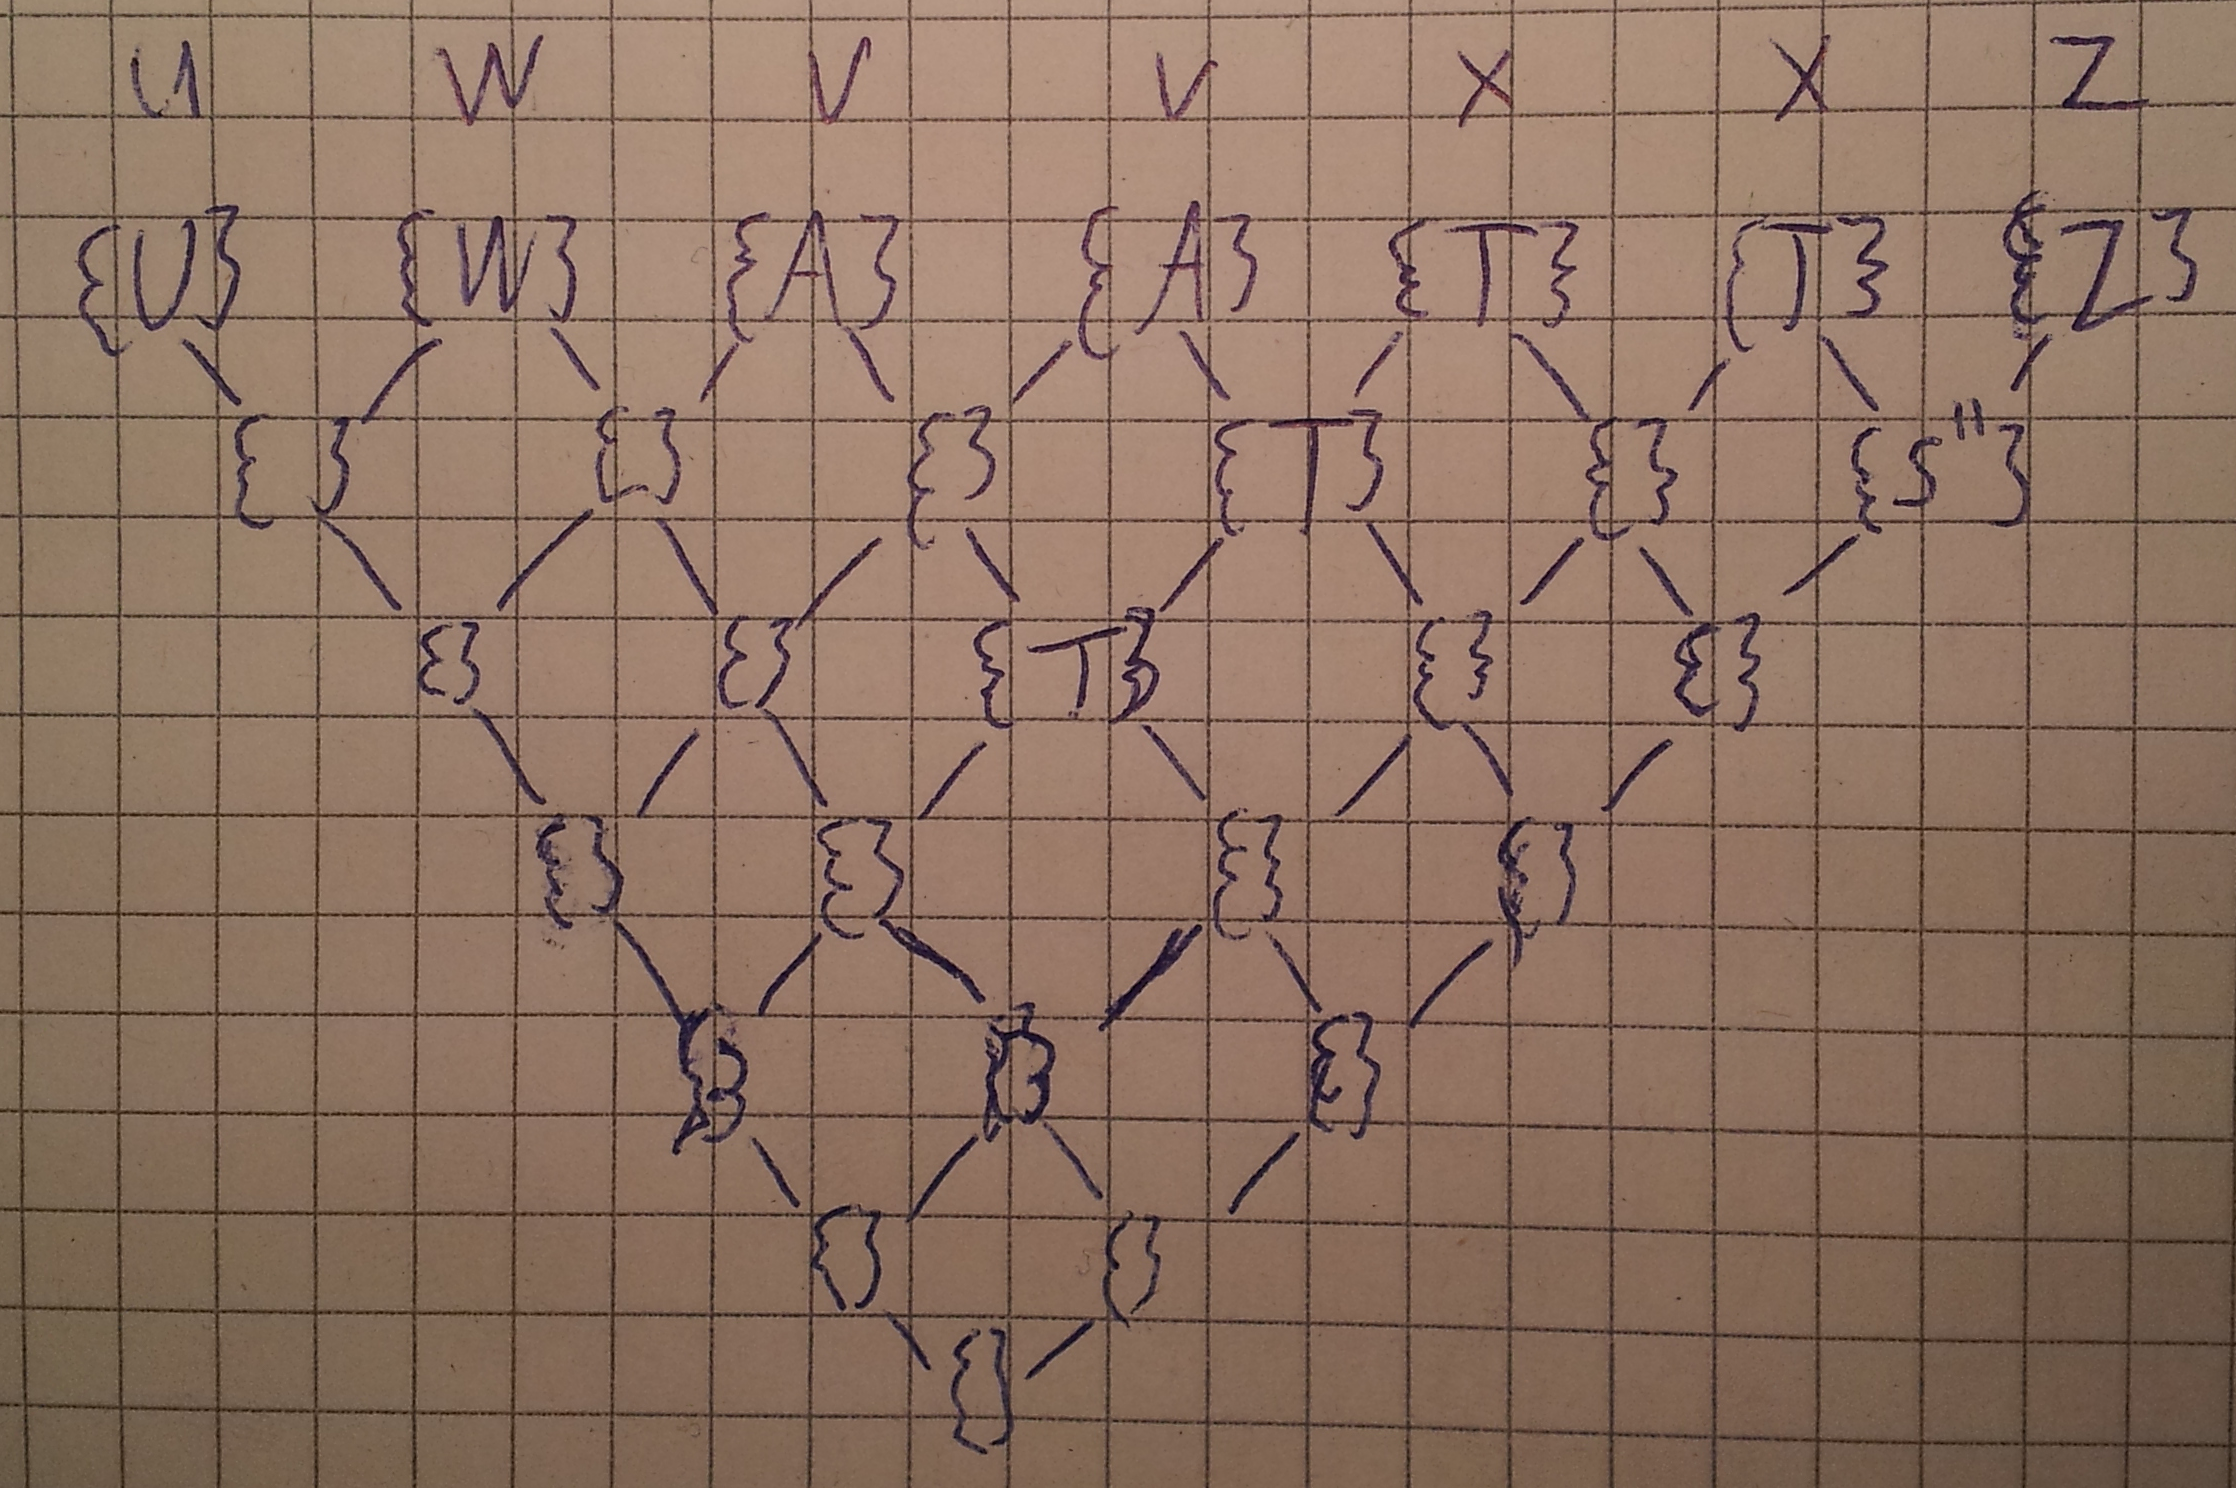
\includegraphics[width=300pt]{6_4_c_1.png}

Also ist $uwvvxxz \not\in L(G_{1})$, weil die Spitze der Pyramide leer ist.

Man ersetze $P_{2}$ mit
\begin{align*}
  \{ S \rightarrow US', S' \rightarrow BS'', S'' \rightarrow DZ, B \rightarrow BV | w, D \rightarrow EF | EX | x, E \rightarrow EX | x, F \rightarrow y, U \rightarrow u, Z \rightarrow z, V \rightarrow v, X \rightarrow x \}
\end{align*}
um $G_{2}$ in CNF zu bringen.

\includegraphics[width=300pt]{6_4_c_2.png}

Also ist $uwxxz \in L(G_{2})$, weil $S$ in der Spitze der Pyramide ist.

\end{document}